\chapter{Simulation and used memory architectures}

In this chapter I will describe the simulation, environment and agent's reasoning and communication how it is used in later experiments. 

\section{Simulation}

The {\bf simulation} is consists of a set of agents, a set of generators and a set of pieces of food. According to given settings it sequently processes a number of steps, each of which invokes an agents' life step and eventually generating new food.

It can also contains a couple of monitors which observe the environment or agents.

\section{Environment}

The environemt si a two-dimensional space which contains agents and food. Agents can move around and eat the food which is randomly distributed using the food generators. 

\section{Agent}                                                      

As I mentioned previously an agent is an entity in the environment which moves and interact with the world around. The interaction is done through eating food which is a part of the environment and through communication with other agents. The latter one actually changes agents' believes about the environment.

Agent has his needs which influences his desicions as fulfilling his needs keeps him alive. When his internal variables of needs is higher than    

There are four types of agents each of which is different in the way they decide about next step. If one is hungry and sees a food (i.e. there is a piece of food in the sight distance) then they choose to go after this food. If there is no desired food around they go searching for it and that is when differs the agents' actions.

\begin{itemize}
\item \emph{random agent} moves randomly around the environment,
\item \emph{pure reactive agent} sees the whole environment, i.e. they always sees a desired piece of food, 
\item \emph{grid agent} implements a memory based on clustering the space into a grid,
\item \emph{GNG agent} implements a memory based on growing neural gas.
\end{itemize}

\section{Communication}

Apart from what agent sees, there is another way how the agents gather information about the environment. They communicate. It is quite simple way of sharing information. When suggesting an implementation for communication I had to create a unified protocol which could have been used throughout types of agents. Thereby I have tried to have this communication protocol as simple as possible.

Moreover, although all agents have a kind of knowledge about the environment they are not able to answer easily, when they are asked about a specific food location. Since the food appears in environment according to given normal distribution, it is not clear what should be an answer for such question. A couple of possible kinds of answers follows. 

First and the most simple answer might be saying exact X,Y coordinates of the food location as it is stored in agent's mind. Additionaly, there would be a noise added to such an answer, having in mind that the answer should not be perfect and there is always a distortion and inperfection in our answers based on how a person is certain about his answer.
                                              
Another way and possibly more plausible one might be answering by a direction (an angle) with an approximate distance. What both the first suggested XY answer and this one have in common is the answers are hard to combine with the learning method used in GNG memory. GNG works with samples of data which sequently influence the neural network. Both kinds of answers could be used if agents would ask more often or the agent's answer would be a sample of points rightaway.

Having such conditions I have suggested and implemented a communication \ref{solution:decision} where the answer consists of several sample points which are generated according agent's knowledge.

\begin{figure}
  \centering                                
  \includegraphics[scale=0.7]{diagrams/solution/communication.eps}    
  \caption{Simple communication protocol}
  \label{solution:communication}
\end{figure}

\section{Decision making}

While searching for food each type of agents makes the decision where to go next. This process is either done randomly or following ones knowledge of the environment around. A simple diagram of decision making follows.

\begin{figure}
  \centering                                
  \includegraphics[scale=0.7]{diagrams/solution/decision-flowchart.eps}    
  \caption{How the agent decides what to do next}
  \label{solution:decision}
\end{figure}

The diagram \ref{solution:decision} shows how an agents decides what to do. In fact it is common for all types of agents described in this thesis, although the first step "Put known food location into memory" is ommited in case of \emph{random} and \emph{PR agents}.

\section{Memories}

There are two types of memory which should allow agents to improve their lifespan comparing to a random agent. Those are memories based on a growing neural gas and a spatial grid.       

The \emph{GNG memory} uses a self-teaching neural network which has been described in \ref{usedalgo:gng}. The neural network allows the agent to learn approximate location where the food is distributed. Each food kind is given a single neural network which tries to learn the distribution reflecting the data inputs.

The \emph{grid memory} divides the environment into a grid so as to simplify the space and restrict total size of data structure used to describe the space. 




